% !TeX root = RJwrapper.tex
\title{akc: A Tidy Framework for Automatic Knowledge Classification in
R}
\author{by Tian-Yuan Huang, Li Li, and Liying Yang}

\maketitle

\abstract{%
Knowledge classification is an extensive and effective approach for
domain knowledge management. To automatically extract and organize
knowledge from unstructured textualized data is desirable and appealing
in various circumstances. In this paper, the tidy framework for
automatic knowledge classification supported by the \CRANpkg{akc}
package is introduced. With the powerful support from the R ecosystem,
the \CRANpkg{akc} framework could handle multiple procedures in data
science workflow, including text cleaning, keyword extraction, synonyms
consolidation and data presentation. While focusing on bibliometric
analysis, the \CRANpkg{akc} package is extensible to be used in other
contexts. This paper introduces the framework and its features in
detail. Specific examples are given to guide the potential users and
developers to participate in open science of text mining.
}

\hypertarget{introduction}{%
\section{Introduction}\label{introduction}}

Co-word analysis has long been used for knowledge discovery, especially
in the field of library and information science
\citep{callon1986mapping}. Based on co-occurrence relationships between
words or phrases, this method could provide quantitative evidence of
information linkages, mapping the association and evolution of knowledge
over time. In conjunction with social network analysis (SNA), co-word
analysis could be escalated and yield more informative results, such as
topic popularity \citep{huang2019measuring} and knowledge grouping
\citep{khasseh2017intellectual}. Meanwhile, in the area of network
science many community detection algorithms have been proposed to unveil
the topological structure of the network
\citep{Fortunato-627, JavedYounis-626}. These methods have then been
incorporated into the co-word analysis, assisting to group components in
the co-word network. Currently, the co-word analysis based on community
detection is flourishing across various fields, including information
science, social science and medical science
\citep{hu2013co, hu2015research, leung2017bibliometrics, BaziyadShirazi-628}.

For implementation, interactive software applications
(e.g.~\href{http://cluster.cis.drexel.edu/~cchen/citespace/}{CiteSpace}
and \href{https://www.vosviewer.com/}{VOSviewer}) have provided freely
available toolkits for automatic co-word analysis, making this technique
even more popular. Interactive software applications are generally
friendlier to users, but they might not be flexible enough for the whole
data science workflow. In addition, the manual adjustments could be
variant, bringing extra risks to the research reproducibility. In this
paper, we have designed a flexible framework for automatic knowledge
classification, and presented an open software package \CRANpkg{akc}
supported by R ecosystem for implementation. Based on community
detection in co-occurrence network, the package could conduct
unsupervised classification on the knowledge represented by extracted
keywords. Moreover, the framework would handle tasks such as data
cleaning and keyword merging in the upstream of data science workflow,
whereas in the downstream it provides both summarized table and
visualized figure of knowledge grouping. While the package was first
designed for academic knowledge classification in bibliometric analysis,
the framework is rather general, so as to benefit a broader audience who
are interested in text mining, network science and knowledge discovery.

\hypertarget{background}{%
\section{Background}\label{background}}

Classification could be identified as a meaningful clustering of
experience, turning information into structured knowledge
\citep{kwasnik1999role}. In bibliometric research, this method has been
frequently used to group domain knowledge represented by author
keywords, usually listed as a part of co-word analysis, keyword analysis
or knowledge mapping
\citep{he1999knowledge, hu2013co, leung2017bibliometrics, li2017knowledge, wang2018three}.
While all named as (unsupervised) classification or clustering, the
algorithm behind could vary widely. For instance, some researches have
utilized hierarchical clustering to group keywords in into different
themes \citep{hu2015research, khasseh2017intellectual}, whereas the
studies applying VOSviewer have adopted a kind of weighted variant of
modularity-based clustering with a resolution parameter to identify
smaller clusters \citep{van2010software}. In the framework of
\CRANpkg{akc}, we have utilized the modularity-based clustering method
known as community detection in network science
\citep{newman2004fast, Murata2010}. These functions are supported by the
\CRANpkg{igraph} package. Main detection algorithms implemented in
\CRANpkg{akc} include Edge betweenness \citep{girvan2002community},
Fastgreedy \citep{Clauset}, Infomap
\citep{rosvall2007information, rosvall2009map}, Label propagation
\citep{raghavan2007near}, Leading eigenvector \citep{newman2006finding},
Multilevel \citep{Blondel_2008}, Spinglass
\citep{reichardt2006statistical} and Walktrap \citep{pons2005computing}.
The details of these algorithms and their comparisons have been
discussed in the previous studies
\citep{de2014evaluating, yang2016comparative, garg2017comparative, 8620850}.

In practical application, the classification result is susceptible to
data variation. The upstream procedures, such as information retrieval,
data cleaning and word sense disambiguation, play vital roles in
automatic knowledge classification. For bibliometric analysis, the
author keyword field provides valuable source of scientific knowledge.
These keywords are good representation of domain knowledge and could be
used directly for analysis. In addition, such collection of keywords
from papers published in specific fields could provide professional
dictionary for information retrieval, such as keyword extraction from
raw text in the title, abstract and full text of literature. While
focuses on automatic knowledge classification based on community
detection in keyword co-occurrence network, the \CRANpkg{akc} framework
also provides utilities for keyword-based knowledge retrieval, text
cleaning, synonyms merging and data visualization in data science
workflow. These tasks might have different requirements in specific
backgrounds. Currently, \CRANpkg{akc} concentrates on keyword-based
bibliometric analysis of scientific literature. Nonetheless, the R
ecosystem is versatile, and the popular tidy data framework is flexible
to extend to various data science tasks from other different fields
\citep{wickham2014tidy, wickham2016r}, which benefits both end-users and
software developers. In addition, when users have more specific needs in
their tasks, they could easily seek other powerful facilities from R
community. For instance, \CRANpkg{akc} provides functions to extract
keywords using n-grams model (utilizing facilities provided by
\CRANpkg{tidytext}), but skip-gram modelling is not supported currently.
This functionality, on the other hand, could be provided in
\CRANpkg{tokenizers} or \CRANpkg{quanteda} package in R. A greater
picture of natural language processing (NLP) in R could be found in the
\href{https://cran.r-project.org/web/views/NaturalLanguageProcessing.html}{CRAN
Task View: Natural Language Processing}.

\hypertarget{framework}{%
\section{Framework}\label{framework}}

An overview of the framework is given in Figure \ref{fig:fig1}. Note
that the name \CRANpkg{akc} refers to the overall framework for
automatic keyword classification as well as the released R package in
this paper. The whole workflow could be largely divided into four
procedures: (1) Keyword extraction (optional); (2) Keyword
preprocessing; (3) Network construction and clustering; (4) Results
presentation.

\begin{Schunk}
\begin{figure}
\includegraphics[width=1\linewidth,height=0.3\textheight]{fig1} \caption[The design of akc framework]{The design of akc framework.}\label{fig:fig1}
\end{figure}
\end{Schunk}

\begin{enumerate}
\def\labelenumi{(\arabic{enumi})}
\tightlist
\item
  Keyword extraction (optional)
\end{enumerate}

In bibliometric meta-data entries, the textual information of title,
abstract and keyword are usually provided for each paper. If the
keywords were used directly, there is no need to do information
retrieval. Then we could directly skip this procedure and start from
keyword preprocessing. However, sometimes the keyword field is missing,
then we would need to extract the keywords from raw text in the title,
abstract or full text with an external dictionary. At other times, one
might want to get more keywords and their co-occurrence relationships
from each entry. In such case, the keyword field could serve as an
internal dictionary for information retrieval in the provided raw text.

Figure \ref{fig:fig2} has displayed an example of keyword extraction
procedure. First, the raw text would be split into sub-sentences
(clauses), this could suppress the generation of cross-clause n-grams.
Then the sub-sentences would be tokenized into n-grams. The \texttt{n}
could be specified by the users, inspecting the average number of words
in keyword phrases might help decide the maximum number of \texttt{n}.
Finally, a filter is made. Only tokens that have emerged in the
user-defined dictionary are retained for further analysis. The whole
keyword extraction procedure could be implemented automatically with
\texttt{keyword\_extract} function in \CRANpkg{akc}.

\begin{Schunk}
\begin{figure}
\includegraphics[width=1\linewidth,height=0.3\textheight]{fig2} \caption[An example of keyword extraction procedure (the letters are automatically turned to lower case in sentence division)]{An example of keyword extraction procedure (the letters are automatically turned to lower case in sentence division).}\label{fig:fig2}
\end{figure}
\end{Schunk}

\begin{enumerate}
\def\labelenumi{(\arabic{enumi})}
\setcounter{enumi}{1}
\tightlist
\item
  Keyword preprocessing
\end{enumerate}

In practice, the textualized contents are seldom clean enough to
implement analysis directly. Therefore, the upstream data cleaning
process is inevitable. In keyword preprocessing procedure of
\CRANpkg{akc} framework, the cleaning part would take care of some
details in the preprocess, such as convert the letters to lower case and
remove parentheses and contents inside (optional). For merging part,
\CRANpkg{akc} help merge the synonymous phrases according to their
lemmas or stems. While using lemmatization and stem extracting would get
abnormal knowledge tokens, here in \CRANpkg{akc} we have designed a
conversion rule to tackle this problem. We first get the lemmatized or
stemmed form of keywords, then group the keywords by their lemma or
stem, and let the most frequent keyword in the group to represent the
original keyword. This step could be realized by \texttt{keyword\_merge}
function in \CRANpkg{akc} package. An example could be found in Figure
\ref{fig:fig3}. After keyword merging, there might still be too many
keywords included in the analysis, which poses great burden for
computation in the subsequent procedures. Therefore, a filter should be
carried out here, it could exclude the infrequent terms, or extract top
TF-IDF terms, or use any criteria that meets the need. Last, a manual
validation should be carried out to ensure the final data quality.

\begin{Schunk}
\begin{figure}
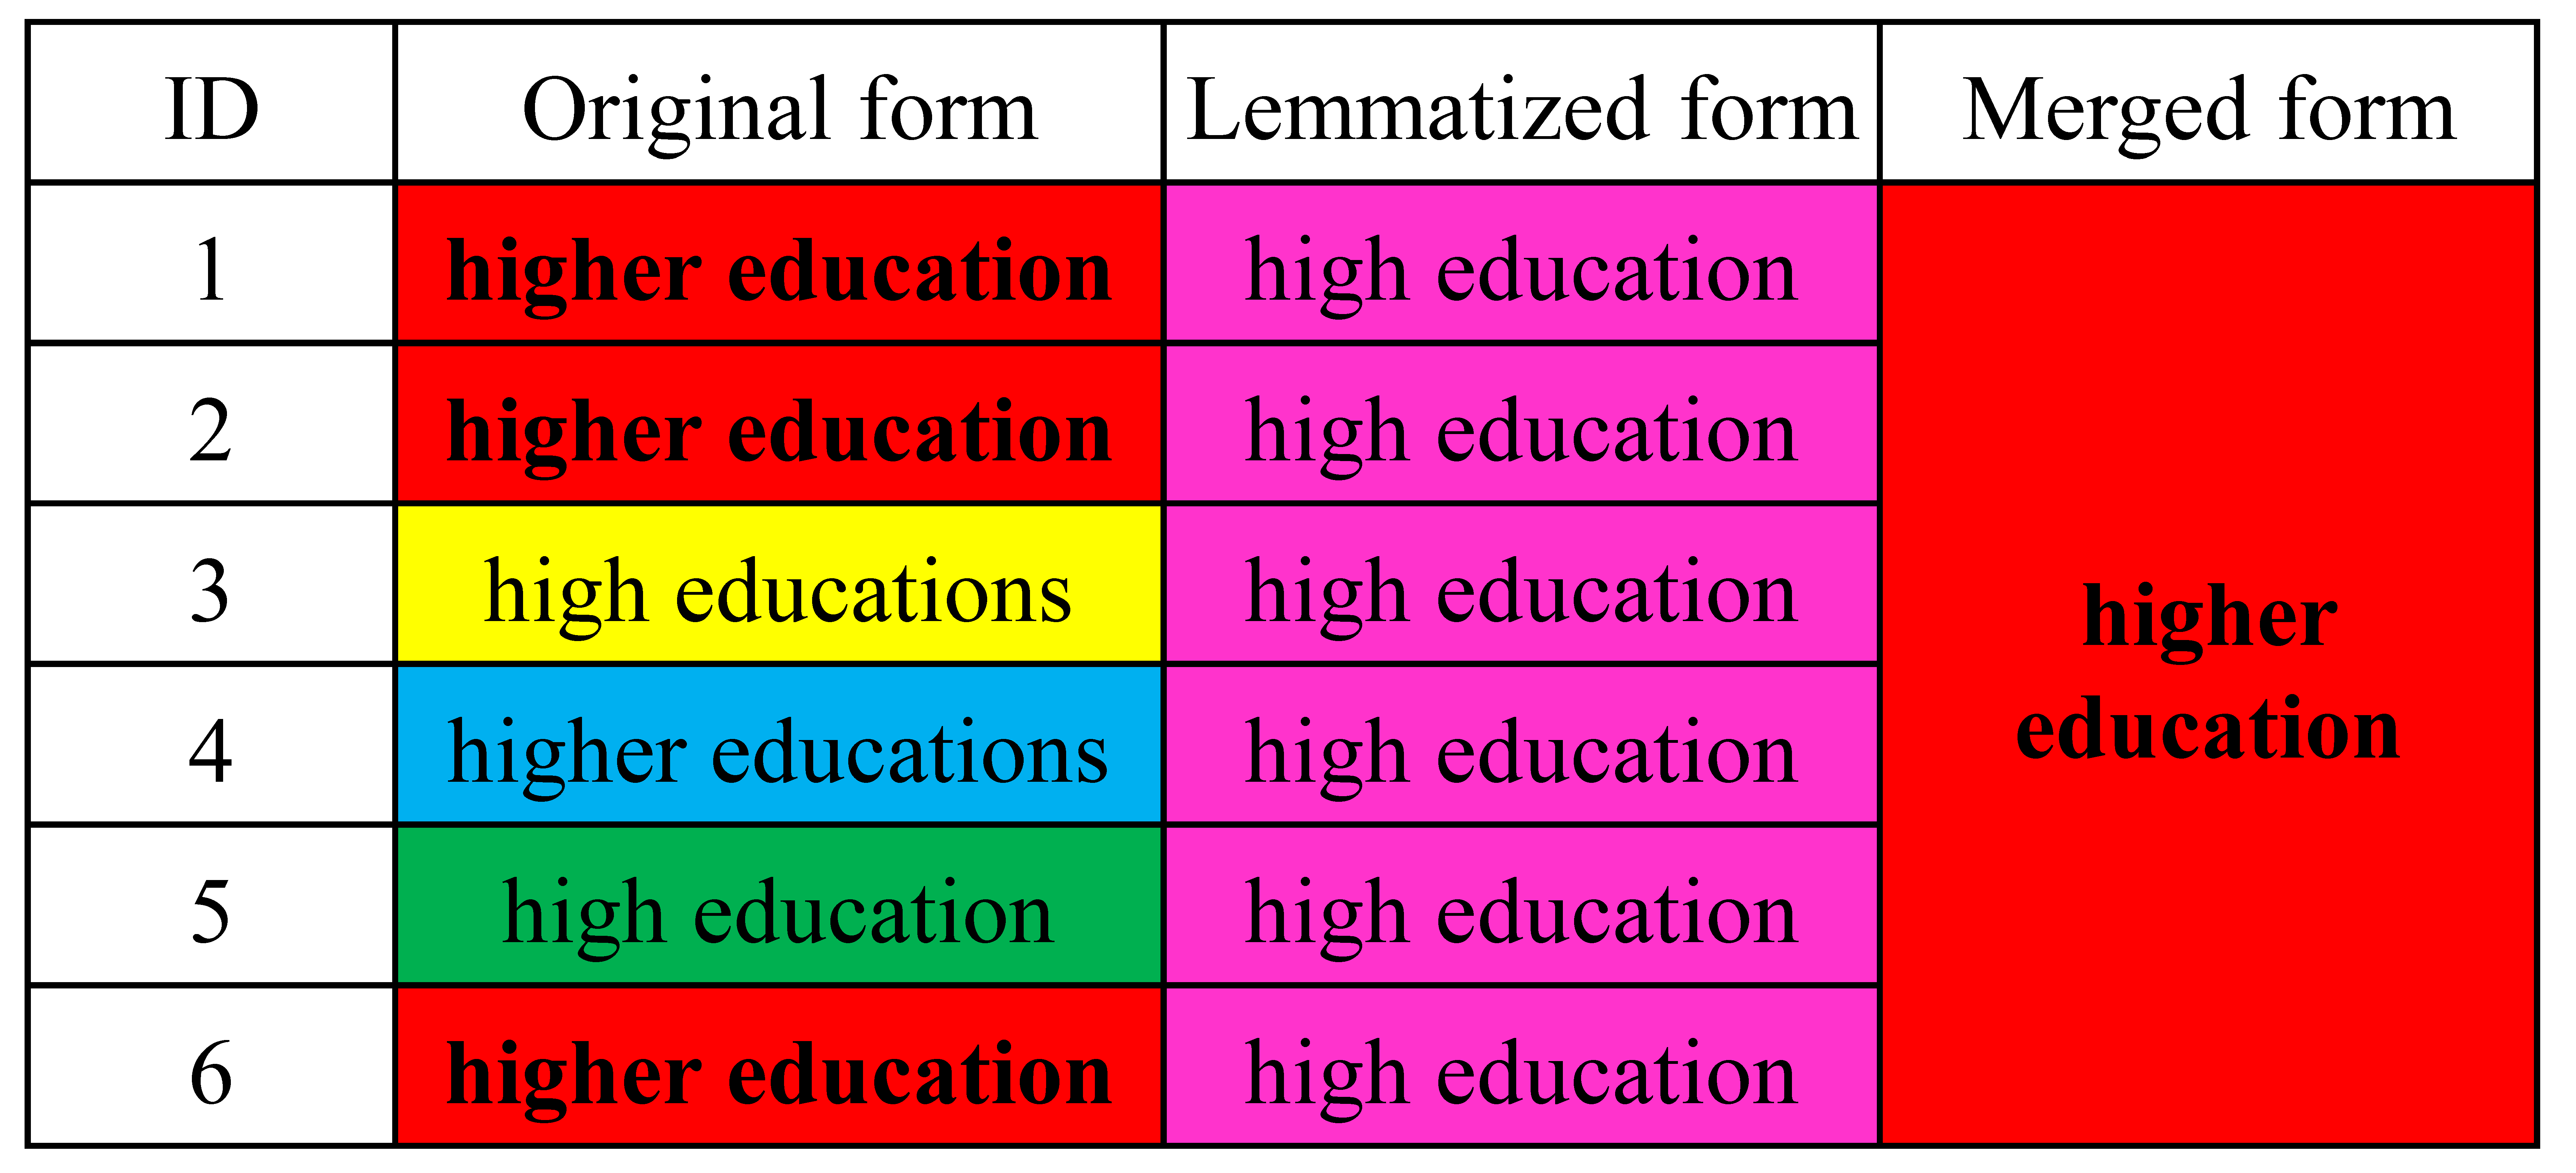
\includegraphics[width=1\linewidth,height=0.25\textheight]{fig3} \caption[An example of keyword merging conversion rule applied in akc]{An example of keyword merging conversion rule applied in akc. The keywords with the same lemma (or stem) would be merged to the highest frequency keyword in the original form.}\label{fig:fig3}
\end{figure}
\end{Schunk}

\begin{enumerate}
\def\labelenumi{(\arabic{enumi})}
\setcounter{enumi}{2}
\tightlist
\item
  Network construction and clustering
\end{enumerate}

Based on keyword co-occurrence relationship, the keyword pairs would
form an edge list and be used to construct an undirected network. Then
the facilities provided by \CRANpkg{igraph} package would automatically
group the nodes (representing the keywords). This procedure could be
achieved by using \texttt{keyword\_group} function in \CRANpkg{akc}.

\begin{enumerate}
\def\labelenumi{(\arabic{enumi})}
\setcounter{enumi}{3}
\tightlist
\item
  Results presentation
\end{enumerate}

Currently, there are two kinds of output presented by \CRANpkg{akc}. One
is a summarized result, namely a table with group number and keyword
collections (attached with frequency). Another is network visualization,
which has two modes. The local mode provides a keyword co-occurrence
network by group (use facets in \CRANpkg{ggplot2}), whereas the global
mode displays the whole network structure. Note that one might include
huge number of keywords and make a huge network, but in presentation the
users could choose how many keywords from each group to be displayed.
More details could be found in the following sections.

The \CRANpkg{akc} framework could never be built without the powerful
support provided by R community. The \CRANpkg{akc} package was developed
under R environment, and main packages imported to \CRANpkg{akc}
framework include \CRANpkg{data.table} (for high performance computing),
\CRANpkg{dplyr} (for tidy data manipulation), \CRANpkg{ggplot2} (for
data visualization), \CRANpkg{ggraph} (for network visualization),
\CRANpkg{ggwordcloud} (for word cloud visualization), \CRANpkg{igraph}
(for network analysis), \CRANpkg{stringr} (for string operations),
\CRANpkg{textstem} (for lemmatizing and stemming), \CRANpkg{tidygraph}
(for network data manipulation) and \CRANpkg{tidytext} (for tidy
tokenization). Getting more understandings on these R packages could
help users utilize more alternative functions, so as to complete more
specific and complex tasks. Hopefully, the users might also become
potential developers of the \CRANpkg{akc} framework in the future.

\hypertarget{example}{%
\section{Example}\label{example}}

This section shows how \CRANpkg{akc} can be used in a real case. A
collection of bibliometric data of \emph{R Journal} from 2009 to 2021 is
used in this example. The data of this example can be accessed in the
\href{https://github.com/hope-data-science/RJ_akc}{GitHub repository}.
Only \CRANpkg{akc} package would be used in this workflow, first we
would load the package and import the data in the R environment.

\begin{Schunk}
\begin{Sinput}
library(akc)
rj_bib = readRDS("./rj_bib.rds")
rj_bib
\end{Sinput}
\begin{Soutput}
#> # A tibble: 568 x 4
#>       id title                                                    abstract  year
#>    <int> <chr>                                                    <chr>    <dbl>
#>  1     1 Aspects of the Social Organization and Trajectory of th~ Based p~  2009
#>  2     2 asympTest: A Simple R Package for Classical Parametric ~ asympTe~  2009
#>  3     3 ConvergenceConcepts: An R Package to Investigate Variou~ Converg~  2009
#>  4     4 copas: An R package for Fitting the Copas Selection Mod~ This ar~  2009
#>  5     5 Party on!                                                Random ~  2009
#>  6     6 Rattle: A Data Mining GUI for R                          Data mi~  2009
#>  7     7 sos: Searching Help Pages of R Packages                  The sos~  2009
#>  8     8 The New R Help System                                    Version~  2009
#>  9     9 Transitioning to R: Replicating SAS, Stata, and SUDAAN ~ Statist~  2009
#> 10    10 Bayesian Estimation of the GARCH(1,1) Model with Studen~ This no~  2010
#> # ... with 558 more rows
\end{Soutput}
\end{Schunk}

\texttt{rj\_bib} is a data frame with 4 columns, including \emph{id}
(Paper ID), \emph{title} (Title of paper), \emph{abstract} (Abstract of
paper) and \emph{year} (Publcation year of paper). Papers in \emph{R
Journal} do not contain keyword field, thus we would have to extract the
keywords from the title or abstract field (first step in Figure
\ref{fig:fig1}). Here in our case, we would use abstract field as our
data source. In addition, we would need a user-defined dictionary to
extract the keywords, otherwise all the n-grams (meaningful or
meaningless) would be extracted and the results would include redundant
noise.

\begin{Schunk}
\begin{Sinput}
# import the user-defined dictionary
rj_user_dict = readRDS("./rj_user_dict.rds")
rj_user_dict
\end{Sinput}
\begin{Soutput}
#> # A tibble: 627 x 1
#>    keyword            
#>    <chr>              
#>  1 seasonal-adjustment
#>  2 unit roots         
#>  3 transformations    
#>  4 decomposition      
#>  5 combination        
#>  6 integration        
#>  7 competition        
#>  8 regression         
#>  9 accuracy           
#> 10 symmetry           
#> # ... with 617 more rows
\end{Soutput}
\end{Schunk}

Note that the dictionary should be a data.frame with only one column
named ``keyword''. The user can also use \texttt{make\_dict} function to
build the dictionary data.frame with a string vector. This function
removes duplicated phrases, turn them to lower case and sort them, which
potentially improving the efficiency for the following processes.

\begin{Schunk}
\begin{Sinput}
rj_dict = make_dict(rj_user_dict$keyword)
\end{Sinput}
\end{Schunk}

With the bibliometric data (\texttt{rj\_bib}) and dictionary data
(\texttt{rj\_dict}), we could start the workflow provided in Figure
\ref{fig:fig1}.

\begin{enumerate}
\def\labelenumi{(\arabic{enumi})}
\tightlist
\item
  Keyword extraction
\end{enumerate}

In this step, we need a bibliometric data table with simply two
informative columns, namely paper ID (\emph{id}) and the raw text field
(in our case \emph{abstract}). The parameter \emph{dict} is also
specified to extract only keywords emerging in the user-defined
dictionary. The implementation is very simple.

\begin{Schunk}
\begin{Sinput}
rj_extract_keywords = rj_bib %>% 
  keyword_extract(id = "id",text = "abstract",dict = rj_dict)
\end{Sinput}
\end{Schunk}

By default, only phrases range 1 to 4 in length are included as
extracted keywords. The user can update this range using parameters
\texttt{n\_min} and \texttt{n\_max} in \texttt{keyword\_extract}
function. These is also a \texttt{stopword} parameter, allowing users to
exclude specific keywords in the extracted phrases. The output of
\texttt{keyword\_extract} is a pretty displayed data.frame
(tibble,\texttt{tbl\_df} class provided by \CRANpkg{tibble} package)
with two columns, namely paper ID (\emph{id}) and the extracted keyword
(\emph{keyword}).

\begin{enumerate}
\def\labelenumi{(\arabic{enumi})}
\setcounter{enumi}{1}
\tightlist
\item
  Keyword preprocessing
\end{enumerate}

For the preprocessing part, \texttt{keyword\_clean} and
\texttt{keyword\_merge} would be implemented. In the cleaning part, the
\texttt{keyword\_clean} function would: 1) Split the text with
separators (If no separators exist, skip); 2) Remove the contents in the
parentheses (including the parentheses, optional); 3) Remove white
spaces from start and end of string and reduces repeated white spaces
inside a string; 4) Remove all the null character string and pure number
sequences (optional); 5) Convert all letters to lower case; 6)
Lemmatization (optional). The merging part has been illustrated in the
previous section, thus would not be explained again. In the tidy
workflow, the preprocessing could be implemented via:

\begin{Schunk}
\begin{Sinput}
rj_cleaned_keywords = rj_extract_keywords %>% 
  keyword_clean() %>% 
  keyword_merge()
\end{Sinput}
\end{Schunk}

No parameters are used in these functions because \CRANpkg{akc} has been
designed to input and output tibbles with consistent column names. If
the users have data tables with different column names, specify them in
arguments (\texttt{id} and \texttt{keyword}) provided by the functions.
More details could be found in the help document (use
\texttt{?keyword\_clean} and \texttt{?keyword\_merge} in the console).

\begin{enumerate}
\def\labelenumi{(\arabic{enumi})}
\setcounter{enumi}{2}
\tightlist
\item
  Network construction and clustering
\end{enumerate}

To construct a keyword co-occurrence network, only a data table with two
columns (with paper ID and keyword) is needed. All the details have been
taken care of in the \texttt{keyword\_group} function. However, the user
could specify: 1) the community detection function (use
\texttt{com\_detect\_fun} argument); 2) the filter rule of keywords
according to frequency (use \texttt{top} or \texttt{min\_freq} argument,
or both). In our example, we would use the default settings (utilizing
Fastgreedy algorithm, only top 200 keywords by frequency would be
included).

\begin{Schunk}
\begin{Sinput}
rj_network = rj_cleaned_keywords %>% 
  keyword_group()
\end{Sinput}
\end{Schunk}

The output object \texttt{rj\_network} is a \texttt{tbl\_graph} class
supported by \CRANpkg{tidygraph}, this is a tidy data format containing
the network data. Based on this data, we can present the results in
various forms in the next section.

\begin{enumerate}
\def\labelenumi{(\arabic{enumi})}
\setcounter{enumi}{3}
\tightlist
\item
  Results presentation
\end{enumerate}

Currently, there are two major ways to display the classified results in
\CRANpkg{akc}, namely network and table. A fast way to gain the network
visualization is using \texttt{keyword\_vis} function:

\begin{Schunk}
\begin{Sinput}
rj_network %>% 
  keyword_vis()
\end{Sinput}
\begin{figure}

{\centering 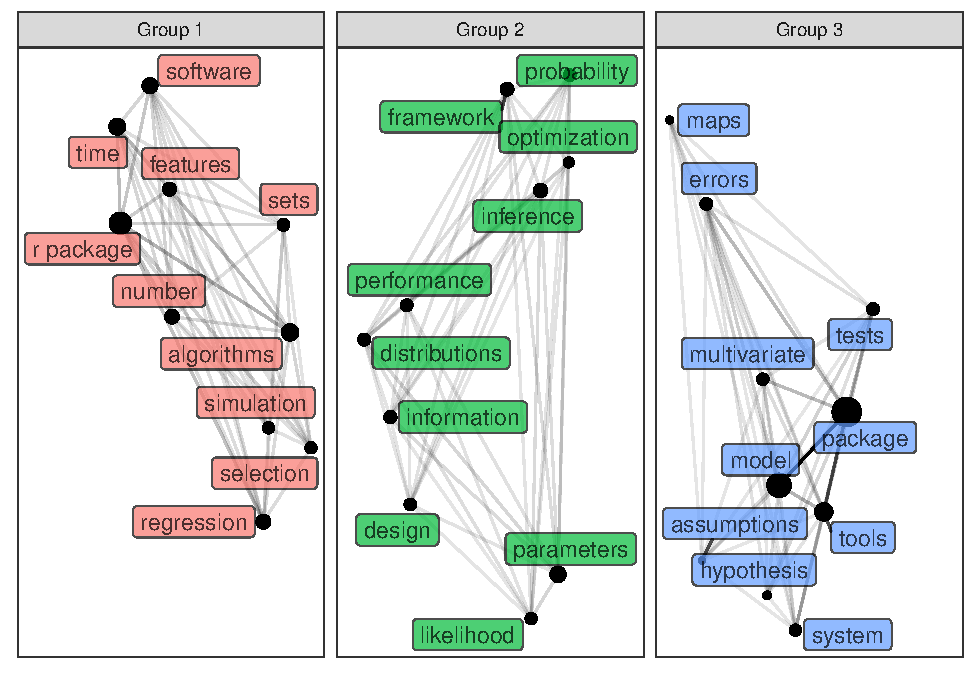
\includegraphics{article_files/figure-latex/fig4-1} 

}

\caption[Network visualization provided by akc]{Network visualization provided by akc.}\label{fig:fig4}
\end{figure}
\end{Schunk}

In Figure \ref{fig:fig4}, the keyword co-occurrence network is clustered
into three groups. The size of nodes is proportional to the keyword
frequency, while the transparency degree of edges is proportional to the
co-occurrence relationship between keywords. For each group, only top 10
keywords by frequency are showed in each facet. If the user wants to dig
into Group 1, \texttt{keyword\_network} could be applied. Also,
\texttt{max\_nodes} parameter could be used to control how many nodes to
be showed (in our case, we show 20 nodes in the visualization displayed
in Figure \ref{fig:fig5}).

\begin{Schunk}
\begin{Sinput}
rj_network %>% 
  keyword_network(group_no = 1,max_nodes = 20) 
\end{Sinput}
\begin{figure}

{\centering 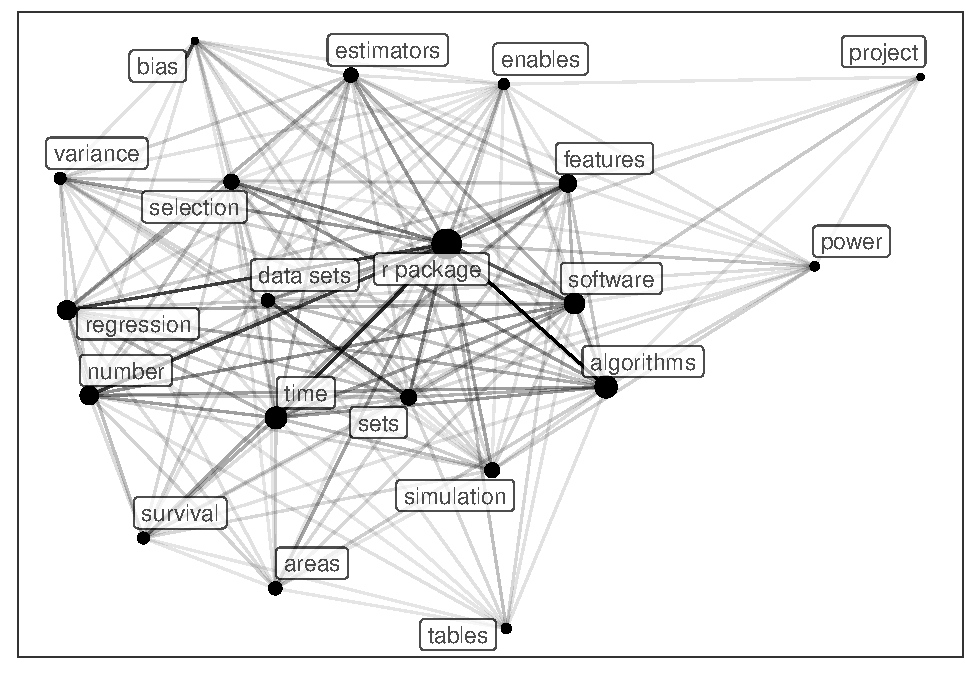
\includegraphics{article_files/figure-latex/fig5-1} 

}

\caption[Focus on one cluster (Group 1) of the network]{Focus on one cluster (Group 1) of the network. Top 20 keywords by frequency are showed.}\label{fig:fig5}
\end{figure}
\end{Schunk}

Another displayed form is using table. This could be implemented by
\texttt{keyword\_table} via:

\begin{Schunk}
\begin{Sinput}
rj_table = rj_network %>% 
  keyword_table() 
\end{Sinput}
\end{Schunk}

This would return a data.frame with two columns (see Table
\ref{tab:tab1-2}), one is the group number, the other is the keywords
(by default, only top 10 keywords by frequency would be displayed, and
the frequency information is attached).

\begin{Schunk}
\begin{table}

\caption{\label{tab:tab1-2}Informative table exported by akc.}
\centering
\fontsize{7}{9}\selectfont
\begin{tabular}[t]{c|>{\centering\arraybackslash}p{10cm}}
\hline
Group & Keywords(TOP 10)\\
\hline
1 & r package (238); algorithms (117); time (109); software (93); regression (75); number (72); features (60); sets (45); selection (41); simulation (40)\\
\hline
2 & parameters (98); inference (65); framework (58); information (51); distributions (48); performance (47); probability (45); design (44); likelihood (41); optimization (31)\\
\hline
3 & package (505); model (310); tools (140); tests (48); errors (46); multivariate (42); system (41); hypothesis (18); maps (16); assumptions (15)\\
\hline
\end{tabular}
\end{table}

\end{Schunk}

Word cloud visualization is also supported by \CRANpkg{akc} via
\CRANpkg{ggwordcloud} package, this could be implemented by using
\texttt{keyword\_cloud} function.

\hypertarget{discussion}{%
\section{Discussion}\label{discussion}}

The core functionality of the akc framework is to automatically group
the knowledge pieces (keywords) using modularity-based clustering.
Because this process is unsupervised, it could be difficult to evaluate
the outcome of classification. Nevertheless, the default setting of
community detection algorithm was selected after empirical tests via
\href{https://cran.r-project.org/web/packages/akc/vignettes/Benchmarking.html}{benchmarking}.
It was found that: 1) Edge betweenness and Spinglass algorithm are most
time-consuming; 2) Edge betweenness and Walktrap algorithm could
potentially find more local clusters in the network; 3) Label
propagation could hardly divide the keywords into groups; 4) Infomap has
high standard deviation of node number across groups. In the end,
Fastgreedy was chosen as the default community detection algorithm in
\CRANpkg{akc}, because its performance is relatively stable, and the
number of groups increases proportionally with the network size.

Though \CRANpkg{akc} currently focuses on automatic knowledge
classification based on community detection in keyword co-occurrence
network, this framework is rather general in many natural language
processing problems. One could utilize part of the framework to complete
some specific tasks, such as word consolidating (using keyword merging)
and n-gram tokenizing (using keyword extraction with a null dictionary),
then export the tidy table and work in another environment. As long as
the data follows the rule of tidy data format \citep{wickham2014tidy},
the \CRANpkg{akc} framework could be easily decomposed and applied in
various circumstances. For instance, by considering the nationalities of
authors as keywords, \CRANpkg{akc} framework could also investigate the
international collaboration behavior in the specific domain.

In the meantime, the \CRANpkg{akc} framework is still in active
development, trying new algorithms to carry out better unsupervised
knowledge classification under the R environment. The expected new
directions include more community detection functions, new clustering
methods, better visualization settings, etc. Note that except for the
topology-based community detection approach considering graph structure
of the network, there is still another topic-based approach considering
the textual information of the network nodes \citep{Ding-629}, such as
hierarchical clustering \citep{Newman-633}, latent semantic analysis
\citep{LandauerFoltz-635} and Latent Dirichlet Allocation
\citep{BleiNg-634}. These methods are also accessible in R, the relevant
packages could be found in the
\href{https://cran.r-project.org/web/views/NaturalLanguageProcessing.html}{CRAN
Task View: Natural Language Processing}. With the tidy framework,
\CRANpkg{akc} could assimilate more nutrition from the modern R
ecosystem, and move forward to create better reproducible open science
schemes in the future.

\hypertarget{conclusion}{%
\section{Conclusion}\label{conclusion}}

In this paper, we have proposed a tidy framework of automatic knowledge
classification supported by a collection of R packages integrated by
\CRANpkg{akc}. While focusing on data mining based on keyword
co-occurrence network, the framework also supports other procedures in
data science workflow, such as text cleaning, keyword extraction and
consolidating synonyms. Though in the current stage it aims to support
analysis in bibliometric research, the framework is quite flexible to
extend to various tasks in other fields. Hopefully, this work could
attract more participants from both R community and academia to get
involved, so as to contribute to the flourishing open science in text
mining.

\hypertarget{acknowledgement}{%
\section{Acknowledgement}\label{acknowledgement}}

This study is funded by The National Social Science Fund of China
``Research on Semantic Evaluation System of Scientific Literature Driven
by Big Data'' (21\&ZD329). This article is created using \pkg{rjtools}
\citep{rjtools2022} in R. The source code and data for reproducing this
paper can be found at:
\url{https://github.com/hope-data-science/RJ_akc}.

\bibliography{article.bib}

\address{%
Tian-Yuan Huang\\
National Science Library, Chinese Academy of Sciences\\%
Beijing, China\\
%
%
\textit{ORCiD: \href{https://orcid.org/0000-0002-4151-3764}{0000-0002-4151-3764}}\\%
\href{mailto:huangtianyuan@mail.las.ac.cn}{\nolinkurl{huangtianyuan@mail.las.ac.cn}}%
}

\address{%
Li Li\\
National Science Library, Chinese Academy of Sciences\\%
Beijing, China\\
%
%
%
\href{mailto:lili2020@mail.las.ac.cn}{\nolinkurl{lili2020@mail.las.ac.cn}}%
}

\address{%
Liying Yang\\
National Science Library, Chinese Academy of Sciences\\%
Beijing, China\\
%
%
%
\href{mailto:yangly@mail.las.ac.cn}{\nolinkurl{yangly@mail.las.ac.cn}}%
}
